\documentclass[10pt,a4paper]{article}
\usepackage[T1]{fontenc}
\usepackage[utf8]{inputenc}
\usepackage[dutch]{babel}
\usepackage[margin=20mm,top=18mm,bottom=18mm,headheight=18pt,headsep=5mm]{geometry}
\usepackage{amsmath,amssymb}
\usepackage{graphicx}
\usepackage{booktabs}
\usepackage{xcolor}
\usepackage{fancyhdr}
\usepackage[font=small,labelfont=bf,skip=3pt]{caption}
\usepackage{enumitem}
\usepackage{float}
\setlist{itemsep=1pt,topsep=3pt,parsep=0pt}
\setlength{\parskip}{4pt}
\setlength{\parindent}{0pt}
\definecolor{qdat}{HTML}{1a1a1a}
\graphicspath{{resultaten/}{../Frame-analyse/}}

% automatisch gegenereerd door onderzoek_lijnvolgen.m -- niet met de hand aanpassen
\newcommand{\LijnBaseEmax}{62}
\newcommand{\LijnBaseJit}{0{,}46}
\newcommand{\LijnBaseKp}{2291}
\newcommand{\LijnBaseOk}{30/30}
\newcommand{\LijnBaseTpar}{124{,}9}
\newcommand{\LijnBestBereik}{28{,}6}
\newcommand{\LijnBestEmax}{42}
\newcommand{\LijnBestJit}{0{,}018}
\newcommand{\LijnBestKd}{0{,}11}
\newcommand{\LijnBestKp}{226}
\newcommand{\LijnBestKster}{464}
\newcommand{\LijnBestKv}{0{,}68}
\newcommand{\LijnBestL}{45}
\newcommand{\LijnBestOk}{30/30}
\newcommand{\LijnBestPwmMm}{6{,}6}
\newcommand{\LijnBestSteek}{12{,}7}
\newcommand{\LijnBestTaud}{34}
\newcommand{\LijnBestTpar}{73{,}0}
\newcommand{\LijnBestVmax}{0{,}47}
\newcommand{\LijnBestVpar}{0{,}42}
\newcommand{\LijnDuur}{58}
\newcommand{\LijnEbereik}{28{,}5}
\newcommand{\LijnLmax}{92}
\newcommand{\LijnLmin}{120}
\newcommand{\LijnNkand}{76}
\newcommand{\LijnNrun}{30}
\newcommand{\LijnNtest}{10}
\newcommand{\LijnRkrap}{15}
\newcommand{\LijnSteekUni}{12{,}7}
\newcommand{\LijnTapeTienE}{33}
\newcommand{\LijnTapeTienOk}{100}
\newcommand{\LijnTaum}{83}
\newcommand{\LijnTd}{85}
\newcommand{\LijnVbocht}{0{,}35}
\newcommand{\LijnVnul}{0{,}47}

% automatisch gegenereerd door onderzoek_obstakels.m -- niet met de hand aanpassen
\newcommand{\ObstAlfaKruisHi}{32}
\newcommand{\ObstAlfaKruisLo}{16}
\newcommand{\ObstBbeschA}{58}
\newcommand{\ObstBbeschB}{118}
\newcommand{\ObstBestAfst}{8{,}7}
\newcommand{\ObstBestAlfa}{43}
\newcommand{\ObstBestDslow}{29}
\newcommand{\ObstBestDstop}{28}
\newcommand{\ObstBestDzij}{45}
\newcommand{\ObstBestEcho}{nee}
\newcommand{\ObstBestEnc}{met encoders}
\newcommand{\ObstBestExtra}{46}
\newcommand{\ObstBestKzij}{1{,}0}
\newcommand{\ObstBestNf}{1}
\newcommand{\ObstBestOpst}{kruis2}
\newcommand{\ObstBestPr}{47}
\newcommand{\ObstBestPtest}{51}
\newcommand{\ObstBestPtestR}{46}
\newcommand{\ObstBestPv}{51}
\newcommand{\ObstBestPvHi}{61}
\newcommand{\ObstBestPvLo}{41}
\newcommand{\ObstBestRem}{tegenstroom}
\newcommand{\ObstBestStrat}{draai}
\newcommand{\ObstBestTmeas}{69}
\newcommand{\ObstBestV}{0{,}14}
\newcommand{\ObstBestWdraai}{1{,}2}
\newcommand{\ObstBestZonder}{kruis2}
\newcommand{\ObstBestZonderPv}{68}
\newcommand{\ObstDekKruisOpt}{100}
\newcommand{\ObstDekRechtA}{40}
\newcommand{\ObstDekRechtB}{82}
\newcommand{\ObstDeltaMax}{1{,}1}
\newcommand{\ObstDnodigA}{54}
\newcommand{\ObstDnodigB}{27}
\newcommand{\ObstDraaiMax}{19}
\newcommand{\ObstDraaiMin}{-30}
\newcommand{\ObstDraaiU}{23}
\newcommand{\ObstDuur}{32}
\newcommand{\ObstEncStap}{5{,}3}
\newcommand{\ObstGamDertig}{19}
\newcommand{\ObstGamZestig}{55}
\newcommand{\ObstHuidigPr}{0}
\newcommand{\ObstHuidigPv}{0}
\newcommand{\ObstHuidigT}{6}
\newcommand{\ObstKortPv}{55}
\newcommand{\ObstNkand}{70}
\newcommand{\ObstNtrain}{16}
\newcommand{\ObstNval}{100}
\newcommand{\ObstRcirkel}{1{,}1}
\newcommand{\ObstRvoor}{97}
\newcommand{\ObstRzwaai}{148}
\newcommand{\ObstRzwaaiKort}{115}
\newcommand{\ObstSremKort}{2{,}5}
\newcommand{\ObstSremRol}{9{,}0}
\newcommand{\ObstSremTegen}{0{,}6}
\newcommand{\ObstTlatDrie}{411}
\newcommand{\ObstTlatEen}{131}
\newcommand{\ObstVmaxDrie}{0{,}36}
\newcommand{\ObstVmaxEen}{0{,}47}
\newcommand{\ObstVmaxRol}{0{,}36}
\newcommand{\ObstWmaxDrie}{1{,}3}
\newcommand{\ObstWmaxEen}{4{,}4}

% terugval als resultaten_obst.tex nog van een oudere run is
\providecommand{\ObstAlfaKruisLo}{16}
\providecommand{\ObstAlfaKruisHi}{30}

\pagestyle{fancy}
\fancyhf{}
\renewcommand{\headrulewidth}{0.4pt}
\fancyhead[L]{\footnotesize Simulatieonderzoek lijnvolgen en obstakeldetectie}
\fancyhead[R]{\raisebox{-1.1mm}{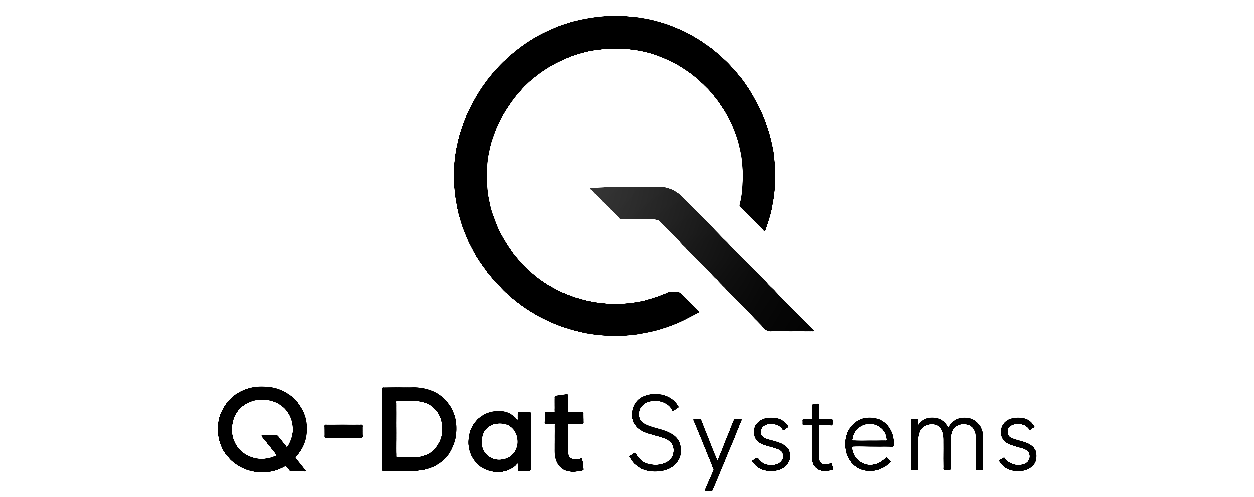
\includegraphics[height=4.5mm]{logo-qdat.png}}}
\fancyfoot[C]{\footnotesize\thepage}

\begin{document}
\thispagestyle{plain}
\noindent
\begin{minipage}[b]{0.5\textwidth}%
  
\includegraphics[height=15mm]{logo-han.png}%
\end{minipage}%
\begin{minipage}[b]{0.5\textwidth}%
  \raggedleft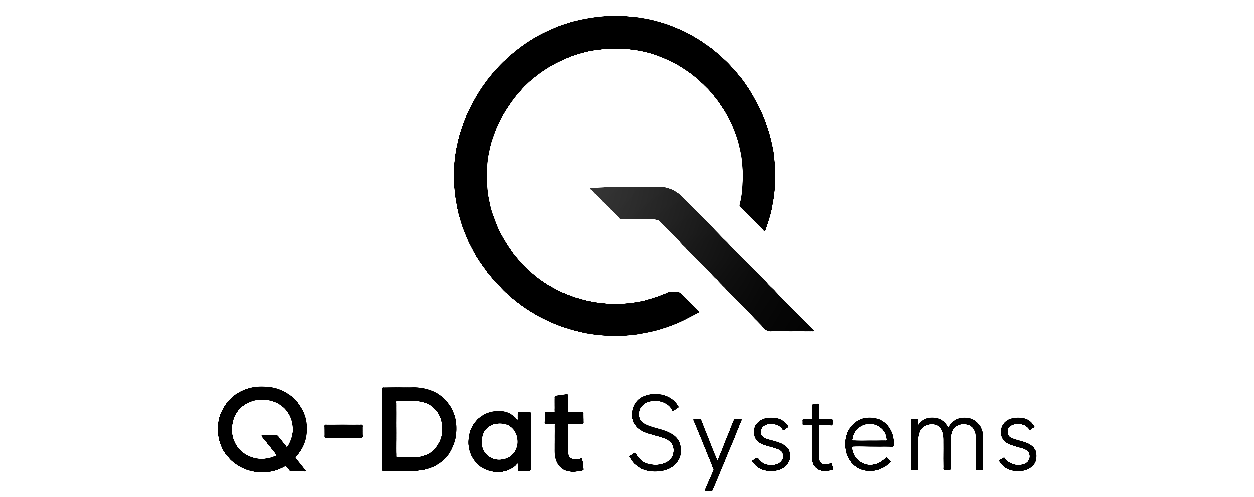
\includegraphics[height=11mm]{logo-qdat.png}%
\end{minipage}

\vspace{3mm}\hrule\vspace{6mm}

{\LARGE\bfseries Simulatieonderzoek lijnvolgen en obstakeldetectie}\\[2mm]
{\large Optimale sensorparameters voor de robot-car (eisen F2 en F3.1)}\\[3mm]
{\small Q-Dat Systems \quad$\cdot$\quad Project 1 Embedded Systems \quad$\cdot$\quad \today\\[1mm]
Opgesteld door \textbf{Claude Opus 5} in opdracht van Tygo Poodt. Alle getallen in dit document
komen rechtstreeks uit \texttt{onderzoek\_lijnvolgen.m} en \texttt{onderzoek\_obstakels.m}.}

\vspace{3mm}\hrule\vspace{4mm}

\textbf{\large Onderzoeksvragen}
\begin{enumerate}[label=\textbf{\arabic*.},leftmargin=8mm]
\item \emph{Lijnvolgen (F3.1).} Hoe ver voor de aandrijfas en met welke onderlinge afstand moeten de
  vier lijnsensoren zitten, en met welke regelaar volgt de auto de lijn het snelst binnen 5~cm?
\item \emph{Obstakels (F2).} Welke opstelling van de HC-SR04 en welk gedrag (snelheid, stopafstand,
  meetfrequentie, filter, remmen, draaien) geven de grootste kans op een botsingsvrije rit van
  2~minuten, zo snel mogelijk?
\end{enumerate}

\vspace{2mm}
\fbox{\parbox{\dimexpr\textwidth-2\fboxsep-2\fboxrule}{%
\textbf{Conclusie.}\quad
\textbf{(1)} De winst zit in de regelaar, niet in de sensorplaatsing. Met de geoptimaliseerde
PD-regelaar ($K_p = \LijnBestKp$~rad/s per m, $v_{\max} = \LijnBestVmax$~m/s) rijdt de auto het
testparcours in \LijnBestTpar~s in plaats van \LijnBaseTpar~s, met ten hoogste \LijnBestEmax~mm
afwijking (eis: 50~mm); de huidige regelaar komt tot \LijnBaseEmax~mm en haalt F3.1 dus niet. De
sensorbalk mag overal tussen 45 en 80~mm voor de aandrijfas zitten, met een steek van 8 tot 15~mm; het
optimum is $L = \LijnBestL$~mm en $s = \LijnBestSteek$~mm ($= w/1{,}5$: de steek die de lijnpositie in
gelijke stappen meet).\quad
\textbf{(2)} Eén HC-SR04 recht vooruit is voor F2 niet genoeg: hij ziet op de stopafstand maar
\ObstBbeschA--\ObstBbeschB~mm van de 143~mm brede neus, en een muur of kist die schuin staat geeft
geen echo. Het huidige ontwerp rijdt in \ObstHuidigPv~\% van de gesimuleerde ritten 2~minuten
zonder botsing. Beide bestelde HC-SR04's gekruist gebruiken (\texttt{kruis2}) werkt duidelijk het
best: in een rommelige ruimte \ObstBestZonderPv~\% botsingsvrij zonder encoders en \ObstBestPv~\% met
(95\%-interval \ObstBestPvLo--\ObstBestPvHi~\%); dat verschil valt binnen de ruis van de optimalisatie.
De kans dat de F2-test (2 van 3 ritten goed) slaagt is daarmee 51 tot 76~\%. De grootste onzekerheid is tot welke hoek een vlak nog een echo geeft; die moet
eerst aan de echte auto gemeten worden.
}}

\section{Opzet: één rekenkern, twee onderzoeken}

Beide simulaties gebruiken dezelfde kern (map \texttt{model/}), zonder graphics, zodat duizenden ritten
parallel kunnen draaien. De 3D-weergave (\texttt{demo\_*.m}) speelt achteraf een doorgerekende rit
af en laadt de carrosserie via \texttt{auto\_3d\_model.m}; een beter 3D-model verandert alleen dat
bestand. Alle maten en aannames staan in \texttt{qdat\_parameters.m}, elk met de bron erbij.

\textbf{Voertuig.} Assenstelsel: oorsprong midden op de aandrijfas, $x$ naar voren, $y$ naar links.
Differentiële aandrijving (Siegwart e.a., hoofdstuk~3):
\begin{equation}
v = \tfrac12 (v_R + v_L), \qquad \omega = \frac{v_R - v_L}{b}, \qquad
\dot x = v\cos\theta,\quad \dot y = v\sin\theta,\quad \dot\theta = \omega
\label{eq:kin}
\end{equation}
\textbf{Motor.} Per wiel een eerste-ordemodel met dode zone $u_{dz}$ en versterking $k_i$
(accuspanning, verschil links/rechts), begrensd op de grip $a_{\text{slip}} = \mu\sigma g$:
\begin{equation}
\tau_m \frac{dv_i}{dt} = k_i\, u_{\text{eff},i}\, v_0 - v_i,\qquad
u_{\text{eff}} = \operatorname{sgn}(u)\,\frac{\max(|u| - u_{dz},\,0)}{1-u_{dz}},\qquad
\tau_m = \frac{J_{eq}\,\omega_0}{\tau_s} = \frac{m r^2 \omega_0}{2\tau_s}
\label{eq:motor}
\end{equation}
Met de motorgegevens uit de frame-analyse ($U_m = 4{,}25$~V aan de klemmen) is $v_0 = \LijnVnul$~m/s
en $\tau_m = \LijnTaum$~ms. De regelaar stuurt een 8-bits PWM-waarde en compenseert de dode zone
met een schatting; de echte dode zone verschilt per run.

\textbf{Onzekerheid.} Een regelaar die alleen werkt in een perfecte simulatie is waardeloos
(Jakobi 1995; Tobin 2017). Elke rit krijgt daarom een eigen trekking van alles wat niet met een
schuifmaat na te meten is (\texttt{variatie\_trekken.m}):

\begin{center}\footnotesize
\begin{tabular}{@{}lll@{}}
\toprule
grootheid & variatie per rit & waarom \\
\midrule
accuspanning (versterking beide motoren) & 85--105~\% & lege tot volle accu \\
verschil motor links/rechts & $\pm$5~\% (lijnvolgen), $\pm$1~\% (F2, gekalibreerd) & goedkope TT-motoren \\
dode zone $u_{dz}$ & 10--22~\% PWM & aanname, meten \\
motortijdconstante $\tau_m$ & 80--130~\% & wrijving tandwielkast \\
effectieve spoorbreedte $b$ & $\pm$3~\% & contactvlak band \\
sensorversterking, -offset, -drempel & 8~\%, 4~\%, $\pm$0{,}08 per kanaal & potmeters LM393 \\
tapebreedte, breedte lichtvlek & $\pm$1~mm, 80--130~\% & \\
halve openingshoek HC-SR04 $\beta$ & 7{,}5--15° & datablad noemt 15° en 30° \\
grootste invalshoek met echo $\gamma_{\max}$ & 30--50° & aanname, \textbf{meten} \\
kans op gemiste echo & 0--4~\% & \\
\bottomrule
\end{tabular}
\end{center}

\textbf{Optimaliseren.} Er is geen Optimization Toolbox nodig: random search met daarna twee rondes
lokale verfijning rond de beste drie kandidaten (\texttt{optimalisatie/}). Bij 5 tot 13 parameters werkt
dat goed en het laat zich perfect paralleliseren; CMA-ES (Hansen 2016) is overwogen maar niet nodig
gebleken. Elke kandidaat rijdt op exact dezelfde banen met dezelfde afwijkingen, zodat verschillen door
de instellingen komen en niet door toeval. Het optimum wordt daarna getoetst op banen en ruimtes die de
optimizer nooit heeft gezien.

% =====================================================================
\section{Simulatie 1: lijnvolgen (F3.1)}

\subsection{Sensormodel}
Een TCRT5000 kijkt naar een lichtvlek op de vloer. Benader die vlek als een Gaussische vlek met breedte
$\sigma$; het deel dat op tape van breedte $w$ valt, als het midden van de vlek op afstand $d$ van de
tapehartlijn staat, is
\begin{equation}
c(d) = \tfrac12\left[\operatorname{erf}\!\left(\frac{w/2 - d}{\sqrt2\,\sigma}\right)
+ \operatorname{erf}\!\left(\frac{w/2 + d}{\sqrt2\,\sigma}\right)\right]
\label{eq:dekking}
\end{equation}
Het signaal is $s_i = g_i\,c(d_i) + o_i + \text{ruis}$; de comparator van de module maakt daar
$b_i = [s_i > \vartheta_i]$ van. De positie van de lijn onder de balk is het zwaartepunt van de actieve
sensoren, $\hat e = \sum y_i b_i / \sum b_i$. Analoog uitlezen (ADC) gebruikt $s_i$ zelf als gewicht.

\subsection{Steek: de lijnpositie in gelijke stappen meten}
Bij drempel $\tfrac12$ en $\sigma \ll w$ springt sensor $i$ om bij $e = y_i \pm w/2$. Met
$y_i = \bigl(i - \tfrac{N+1}{2}\bigr)s$ zijn dat twee roosters met steek $s$, ten opzichte van elkaar
verschoven over $w \bmod s$. De stappen in $\hat e$ zijn dus afwisselend $w \bmod s$ en
$s - (w \bmod s)$, en alleen gelijk ($= s/2$) als
\begin{equation}
\frac{w}{s} = k + \tfrac12 \quad\Longrightarrow\quad s = \frac{w}{1{,}5} = \LijnSteekUni~\text{mm}
\quad (k = 1,\ w = 19~\text{mm}),
\qquad e_{\text{bereik}} = \frac{(N-1)\,s}{2} + \frac{w}{2}
\label{eq:steek}
\end{equation}
Is $s > w$, dan ontstaan er posities waar geen enkele sensor de lijn ziet. De huidige plaatsing
($-22, -7, 7, 22$~mm) geeft stappen van 4 tot 15~mm (figuur~\ref{fig:sensor}b).

\begin{figure}[H]
\centering
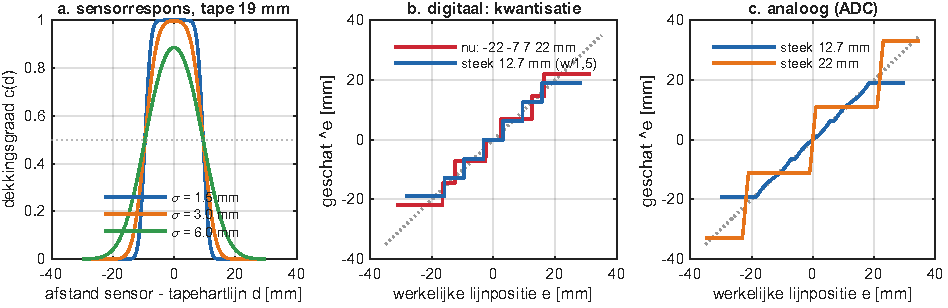
\includegraphics[width=\textwidth]{lijn_sensormodel.pdf}
\caption{(a) Dekkingsgraad \eqref{eq:dekking}. (b) Geschatte tegen werkelijke lijnpositie bij
digitaal uitlezen: de huidige plaatsing meet in ongelijke stappen, steek $w/1{,}5$ in gelijke.
(c) Analoog uitlezen interpoleert tussen de sensoren.}
\label{fig:sensor}
\end{figure}

\subsection{Waarom de sensorbalk vóór de as moet zitten: een lineair model}
Zij $e$ de zijdelingse afwijking van de aandrijfas ten opzichte van de lijn, $\psi$ de koersfout en
$\kappa$ de kromming van de lijn. Een sensorbalk op afstand $L$ voor de as meet
$e_s \approx e + L\psi - \tfrac12 L^2\kappa$. Met $\dot e = v\psi$, $\dot\psi = \omega - v\kappa$ en een
P-regelaar $\omega = -K e_s$ volgt
\begin{equation}
\ddot e + K L\,\dot e + K v\, e = v\kappa\left(\tfrac12 K L^2 - v\right)
\;\Longrightarrow\;
\omega_n = \sqrt{Kv},\quad \zeta = \frac{L}{2}\sqrt{\frac{K}{v}},\quad
e_{ss} = \kappa\left(\frac{L^2}{2} - \frac{v}{K}\right)
\label{eq:lin}
\end{equation}
De look-ahead $L$ werkt dus als demping, net als een D-term. De keuze
\begin{equation}
K^* = \frac{2v}{L^2} \quad\Longrightarrow\quad e_{ss} = 0 \ \text{in elke bocht},\qquad
\zeta = \frac{1}{\sqrt2},\qquad \omega_n = \frac{\sqrt2\, v}{L}
\label{eq:kster}
\end{equation}
geeft tegelijk nul blijvende fout in een bocht én de klassieke optimale demping. Twee grenzen
bepalen het venster voor $L$ (figuur~\ref{fig:venster}):
\begin{itemize}
\item \emph{bovengrens}: in de krapste bocht (straal $R$) moet de lijn onder de balk blijven,
  $L^2/(2R) \le e_{\text{bereik}}$, dus $L \le \sqrt{2Re_{\text{bereik}}}$; bij $R = \LijnRkrap$~cm en
  $e_{\text{bereik}} = \LijnEbereik$~mm is dat \LijnLmax~mm;
\item \emph{ondergrens}: de lus mag niet sneller willen reageren dan motor en bemonstering toelaten.
  Met de totale vertraging $T_d = \tau_m + T_s/2 = \LijnTd$~ms en de vuistregel $\omega_n T_d \le 0{,}3$
  wordt $L \ge \sqrt2\, v T_d / 0{,}3$, bij 0,3~m/s \LijnLmin~mm.
\end{itemize}
Bij 0,3~m/s sluiten die grenzen elkaar uit: in krappe bochten moet de auto langzamer. Dat doet de
snelheidswet $v = \max\!\bigl(v_{\min},\, v_{\max}(1 - k_v|\hat e|/e_{\text{bereik}})\bigr)$.
Daarnaast begrenst de motor zelf de bochtsnelheid: het buitenwiel rijdt $v(1 + b/2R) \le v_0$, dus
$v \le v_0/(1 + b/2R) = \LijnVbocht$~m/s bij $R = \LijnRkrap$~cm.
Het simulatie-optimum ($L = \LijnBestL$~mm) ligt onder de vuistregel-ondergrens: de lus is minder
gedempt dan $\zeta = 1/\sqrt2$ en slingert licht om de lijn (ongeveer $\pm$7~mm,
figuur~\ref{fig:tijd}). De kostfunctie accepteert dat in ruil voor snelheid.

\begin{figure}[H]
\centering
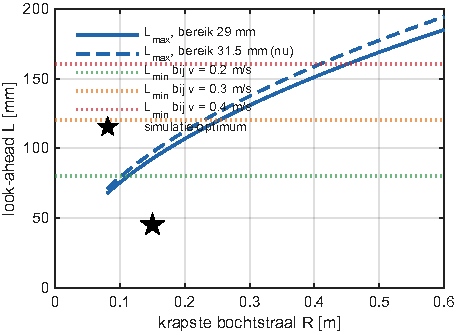
\includegraphics[width=0.55\textwidth]{lijn_venster.pdf}
\caption{Venster voor de look-ahead $L$: boven de blauwe lijn raakt de auto de lijn kwijt in een bocht
met straal $R$, onder een stippellijn reageert de lus te snel voor motor en bemonstering.}
\label{fig:venster}
\end{figure}

\subsection{Optimalisatie}
Kost per rit (\texttt{lijn\_kost.m}), lager is beter:
\begin{equation}
J = \frac{T v_0}{L_{\text{baan}}}
+ \lambda_e \max\!\left(0, \frac{e_{\max}}{e_{\text{toel}}} - 1\right)
+ \lambda_k f_{\text{kwijt}} + \lambda_j\, j
\label{eq:jlijn}
\end{equation}
met de genormaliseerde rondetijd ($=1$: hele ronde op volle motorsnelheid), een straf als de grootste
afwijking van de aandrijfas boven $e_{\text{toel}} = 30$~mm komt (F3.1 zegt 50~mm; 20~mm marge voor de
verschillen tussen simulatie en werkelijkheid), de tijdfractie dat de lijn kwijt is en het gejitter van
de PWM. Een mislukte rit kost $10 + 10\,(1-\text{voortgang})$. Per sensoropstelling ($L \times s$, vier
sensoren) worden eerst de vijf regelaarparameters $K_p, K_d, \tau_d, v_{\max}, k_v$ geoptimaliseerd
(\LijnNkand\ kandidaten, vier trainingsbanen, waaronder een met haakse bochten); pas daarna worden
de opstellingen vergeleken. Een opstelling beoordelen met een slecht afgestelde regelaar zegt niets
over de opstelling.

\begin{figure}[H]
\centering
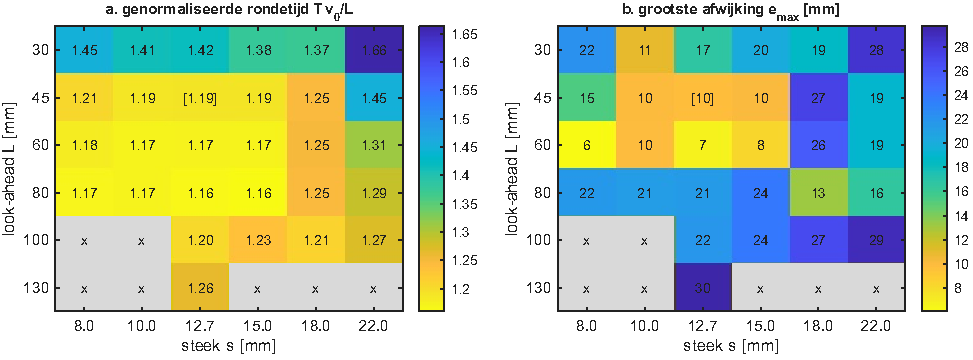
\includegraphics[width=\textwidth]{lijn_kaart.pdf}
\caption{Beste haalbare prestatie per sensoropstelling, elk met een eigen geoptimaliseerde regelaar.
Grijs met $\times$: haalt de eis met marge niet. Tussen haken: het optimum.}
\label{fig:kaart}
\end{figure}

\subsection{Resultaten}
Het optimum ligt op $L = \LijnBestL$~mm en $s = \LijnBestSteek$~mm, met
$K_p = \LijnBestKp$~rad/s per m, $K_d = \LijnBestKd$~rad/s per m/s, een D-filter van
$\tau_d = \LijnBestTaud$~ms, $v_{\max} = \LijnBestVmax$~m/s en $k_v = \LijnBestKv$. Tabel~\ref{tab:val}
toetst vier instellingen op \LijnNtest\ banen die de optimizer niet kende, elk meerdere keren met andere
afwijkingen (\LijnNrun\ ritten per instelling).

\begin{table}[H]
\centering\footnotesize
\begin{tabular}{@{}lrrrrr@{}}
\toprule
 & voltooid & $T$ testparcours & $\bar v$ & $e_{\max}$ & gejitter \\
 & & [s] & [m/s] & [mm] & [PWM/stap] \\
\midrule
huidige sim (teken gecorrigeerd) & 30/30 & 124{,}9 & 0{,}25 & 62 & 0{,}459 \\
huidige sensoren, regelaar geoptimaliseerd & 30/30 & 72{,}8 & 0{,}42 & 43 & 0{,}021 \\
optimale sensoren, analytische $K^*$ & 30/30 & 111{,}6 & 0{,}27 & 12 & 0{,}033 \\
optimum (sensoren + regelaar) & 30/30 & 73{,}0 & 0{,}42 & 42 & 0{,}018 \\
\bottomrule
\end{tabular}

\caption{Validatie. ``Huidige sim'' is de regelaar uit \texttt{RobotCar\_LineFollower\_Sim.m}
($K_p = 28$ per gewichtseenheid $\approx \LijnBaseKp$~rad/s per m, 50~Hz) op het realistische motormodel.
Let op: in dat script staat \texttt{omega = -(Kp*pos\_error + Kd*d\_error)} terwijl \texttt{pos\_error}
positief is als de lijn links ligt; zo stuurt de auto van de lijn af (headless nagerekend: na 0,1~s is
hij de lijn kwijt en rijdt hij rondjes). Voor deze vergelijking is het teken omgedraaid.}
\label{tab:val}
\end{table}

Opvallend: de huidige regelaar komt wel rond, maar zijn $K_p$ is zo groot dat elke sensor die omslaat
de wielen van vol links naar vol rechts stuurt (gejitter \LijnBaseJit\ PWM-fractie per stap tegen
\LijnBestJit\ voor het optimum): slecht voor tandwielkast en accu, en traag omdat de auto
slingert. De analytische $K^*$ uit \eqref{eq:kster} alleen is stabiel maar voorzichtig; de optimizer
vindt een hogere snelheid met een snelheidswet die in de bochten terugschakelt.

De sensoropstelling zelf maakt binnen een breed gebied weinig uit: in figuur~\ref{fig:kaart} liggen alle
opstellingen met $L$ tussen 45 en 80~mm en een steek van 8 tot 15~mm binnen 5~\% van elkaar. Pas bij een
steek van 18~mm of meer, een balk vlak bij de as (30~mm) of ver ervoor (100~mm en meer) wordt het
duidelijk slechter. De winst van \LijnBaseTpar\ naar \LijnBestTpar~s komt dan ook vrijwel helemaal uit
de regelaar: met de huidige sensorplaatsing en een geoptimaliseerde regelaar is het resultaat even goed
(tabel~\ref{tab:val}). De huidige regelaar komt wel rond, maar wijkt op de testbanen tot
\LijnBaseEmax~mm af en haalt F3.1 dus niet.

\begin{table}[H]
\centering\footnotesize
\begin{tabular}{@{}lrrr@{}}
\toprule
variant (bij $L = 45$~mm) & kost $J^*$ & $T v_0/L$ & $e_{\max}$ [mm] \\
\midrule
2 sensoren & 1{,}44 & 1{,}25 & 10 \\
3 sensoren & 1{,}36 & 1{,}21 & 12 \\
4 sensoren (optimum) & 1{,}31 & 1{,}19 & 10 \\
5 sensoren & 1{,}29 & 1{,}19 & 11 \\
4 sensoren, analoog & 1{,}24 & 1{,}18 & 11 \\
4, analoog, steek 22 mm & 1{,}40 & 1{,}25 & 17 \\
\bottomrule
\end{tabular}

\caption{Aantal sensoren en analoog uitlezen, elk met een eigen geoptimaliseerde regelaar.}
\label{tab:var}
\end{table}

\begin{figure}[H]
\centering
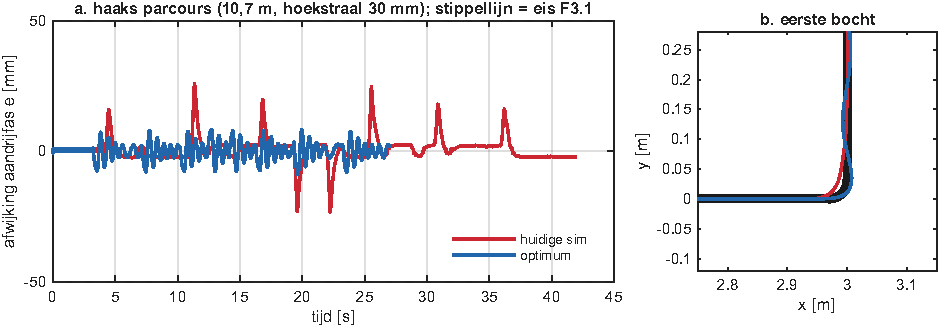
\includegraphics[width=\textwidth]{lijn_tijdreeks.pdf}
\caption{Huidige sim tegen optimum op een parcours met haakse bochten.}
\label{fig:tijd}
\end{figure}

\begin{figure}[H]
\centering
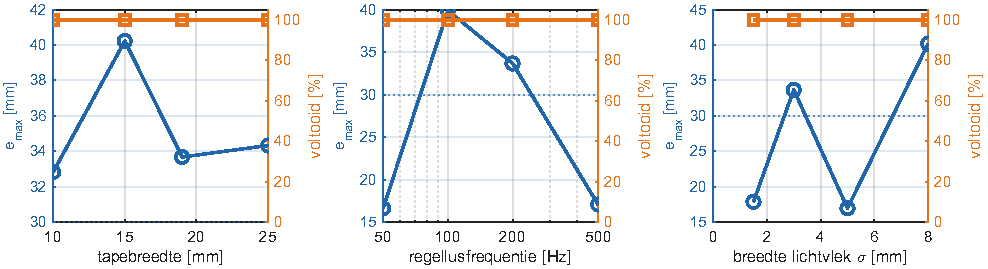
\includegraphics[width=\textwidth]{lijn_robuust.pdf}
\caption{Robuustheid van het optimum op de testbanen. Links: tapebreedte (T9.1 staat 1 tot 2~cm toe).
Bij 10~mm is de steek groter dan de tape, zodat volgens \eqref{eq:steek} gaten ontstaan; de auto komt
toch rond ($e_{\max} = \LijnTapeTienE$~mm, \LijnTapeTienOk~\% voltooid), omdat de lijn door de
look-ahead en de lichtvlek zelden lang in een gat blijft. Midden: regellusfrequentie. Rechts: breedte
van de lichtvlek (hoogte van de sensor). $e_{\max}$ is een slechtste-gevalwaarde over een beperkt aantal
ritten en springt daardoor; geen van de drie laat een duidelijke trend zien.}
\label{fig:rob}
\end{figure}

\subsection{Vertaling naar de Arduino-code}
De regelaar werkt in SI-eenheden; op de ATmega328P (geen FPU) wordt het integerwerk (Wescott 2000).
Per millimeter lijnfout verschuift elk wiel
$\Delta\text{PWM} = K_p \cdot 10^{-3} \cdot \tfrac{b}{2} / v_0 \cdot 255 \approx \LijnBestPwmMm$
PWM-stappen (links erbij, rechts eraf). De D-term op de gemeten positie door een eerste-ordefilter:
$D_k = D_{k-1} + \frac{T_s}{\tau_d + T_s}\bigl((\hat e_k - \hat e_{k-1})/T_s - D_{k-1}\bigr)$; reken
$\hat e$ in hele millimeters en schaal de versterkingen met een macht van 2, dan blijft alles in
\texttt{int16\_t}.

% =====================================================================
\section{Simulatie 2: obstakels herkennen en ontwijken (F2)}

\subsection{Model van de HC-SR04}
De module meet de looptijd van de eerste echo die terugkomt:
\begin{equation}
d = \frac{c\, t_{\text{echo}}}{2},\qquad c = 331{,}3 + 0{,}606\,T~\text{m/s}\quad (T\text{ in °C})
\label{eq:echo}
\end{equation}
In de simulatie is de bundel een waaier van stralen over $[-\beta, \beta]$. Een straal telt alleen als
het vlak dat hij raakt hem terugkaatst: de invalshoek (tussen straal en normaal) moet kleiner zijn dan
$\gamma_{\max}$. Een glad vlak dat te schuin staat kaatst de puls weg, als een spiegel
(Leonard \& Durrant-Whyte 1992); kistranden en binnenhoeken geven wel altijd een zwakke echo. Daarna
komen ruis ($\sigma = 3$~mm), afronding op hele centimeters zoals de Arduino-code doet, 0--4~\% gemiste
echo's, en de timing: een puls om de $T_{\text{meas}} \ge 60$~ms (datablad), het resultaat
$2d/c$ later, bij geen echo pas na de time-out van 38~ms. Twee of drie sensoren vuren om de beurt,
anders horen ze elkaars echo.

\subsection{Remweg en de hoogste snelheid die F2.3 haalt}
Van ``obstakel dichter dan $d_{\text{stop}}$'' tot ``remmen'' zit in het slechtste geval
\begin{equation}
t_{\text{lat}} = n\,T_{\text{meas}}\Bigl(1 + \frac{N_f - 1}{2}\Bigr) + \frac{2d}{c} + \frac{1}{f_s}
\label{eq:tlat}
\end{equation}
($n$ sensoren om de beurt; een mediaanfilter over $N_f$ metingen heeft $(N_f+1)/2$ lage metingen nodig).
Voor één sensor, 60~ms en $N_f = 3$ is dat \ObstTlatEen~ms, voor drie sensoren \ObstTlatDrie~ms. De
remweg hangt af van hoe de L298N remt:
\begin{equation}
s_{\text{rem}} =
\begin{cases}
v\,\tau_m & \text{kortsluitrem (IN1 = IN2, EN hoog)}\\
v\,\tau_m - v_0\tau_m \ln(1 + v/v_0) & \text{tegenstroom, gedurende } t^* = \tau_m\ln(1 + v/v_0)\\
v^2 / (2 a_{\text{rol}}) & \text{uitrollen (EN laag)}
\end{cases}
\label{eq:rem}
\end{equation}
Bij 0,3~m/s is dat \ObstSremKort, \ObstSremTegen\ en \ObstSremRol~cm. F2.3 eist remmen vanaf 20~cm
met 2~cm speling, dus $v\,t_{\text{lat}} + s_{\text{rem}}(v) \le 18$~cm. Met de kortsluitrem geeft dat
$v_{\max} = \ObstVmaxEen$~m/s voor één sensor en \ObstVmaxDrie~m/s voor drie; laat de code de motoren
uitrollen (\texttt{analogWrite(EN, 0)}), dan nog maar \ObstVmaxRol~m/s (figuur~\ref{fig:rem}).

\begin{figure}[H]
\centering
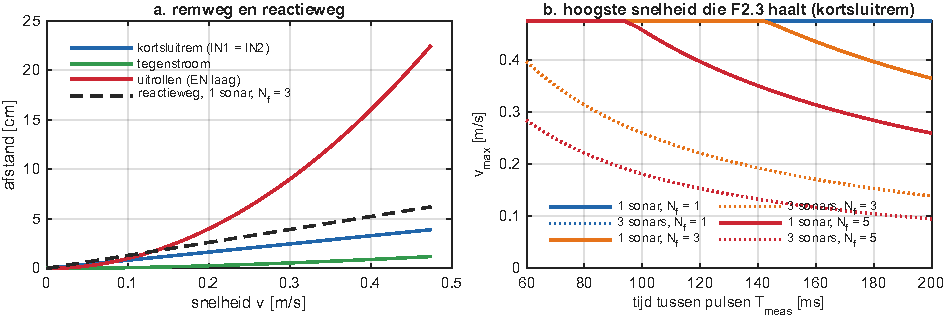
\includegraphics[width=\textwidth]{obst_remweg.pdf}
\caption{(a) Remweg per remmethode en reactieweg. (b) Hoogste snelheid waarbij de auto volgens F2.3
op tijd stilstaat, als functie van de meetperiode en de filterlengte.}
\label{fig:rem}
\end{figure}

\subsection{Welk deel van de auto ziet de sonar?}
Een obstakel op zijafstand $y$ ligt in de bundel van één sensor recht vooruit zolang $x \ge |y|/\tan\beta$.
Nadert de auto, dan valt het er juist \emph{uit}. Op de stopafstand is de beschermde breedte
\begin{equation}
B_{\text{besch}} = 2\, d_{\text{stop}} \tan\beta
\qquad\text{en de hele breedte } B \text{ vraagt}\qquad
d_{\text{stop}} \ge \frac{B/2}{\tan\beta}
\label{eq:besch}
\end{equation}
Bij $d_{\text{stop}} = 22$~cm is $B_{\text{besch}} = \ObstBbeschA$~mm ($\beta = 7{,}5^\circ$) tot
\ObstBbeschB~mm ($\beta = 15^\circ$) van de 143~mm; de hele breedte zien vraagt stoppen op
\ObstDnodigA\ resp.\ \ObstDnodigB~cm, en dat botst met F2.1 (doorrijden zolang 30~cm vrij is). Een
poot of de hoek van een kist die 4--7~cm naast het midden staat, raakt dus de neus zonder ooit gezien
te zijn. Voor meer sensoren geldt: een punt $(x, y)$ wordt door sensor $i$ op $(x_i, y_i)$ met
kijkrichting $\alpha_i$ gezien als
\begin{equation}
\bigl|\operatorname{atan2}(y - y_i,\; x - x_i) - \alpha_i\bigr| \le \beta
\label{eq:kegel}
\end{equation}
Figuur~\ref{fig:dek}a telt voor elke opstelling welk deel van de breedte ergens tussen 5 en 22~cm voor de
sensor in een bundel valt. Twee sensoren ``scheel'' (de linker kijkt naar rechts, \texttt{kruis2}) dekken
het meest: bij elke $\alpha$ tussen \ObstAlfaKruisLo° en \ObstAlfaKruisHi° valt \ObstDekKruisOpt~\% van
de breedte in een bundel, tegen \ObstDekRechtA--\ObstDekRechtB~\% voor één sensor. Twee naar buiten gedraaide sensoren
(\texttt{uit2}) laten het midden open.

\begin{figure}[H]
\centering
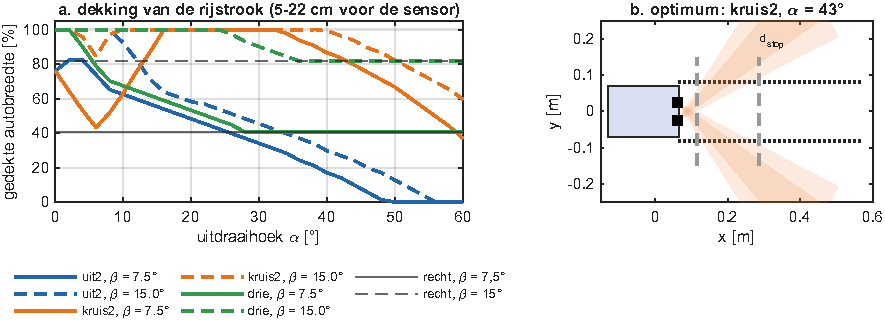
\includegraphics[width=\textwidth]{obst_dekking.pdf}
\caption{(a) Gedekte autobreedte als functie van de uitdraaihoek, uit \eqref{eq:kegel}. (b) Bundels van
het simulatie-optimum ($\beta = 7{,}5^\circ$ en $15^\circ$); stippellijnen: rijstrook.}
\label{fig:dek}
\end{figure}

\subsection{Rechtdoor rijden, draaien en de achterkant}
\textbf{Drift (F2.1).} Draait het rechterwiel een fractie $\delta$ sneller dan gevraagd en het linker
$\delta$ langzamer, dan rijdt de auto een cirkel met straal $b/(2\delta)$ en wijkt hij over een afstand
$s$ af met
\begin{equation}
y(s) = \frac{\delta\, s^2}{b}
\qquad\Longrightarrow\qquad
\delta \le \frac{y_{\max}\, b}{s^2} = \frac{0{,}40 \cdot 0{,}108}{2^2} = \ObstDeltaMax~\%
\label{eq:drift}
\end{equation}
Zonder terugkoppeling moeten de motoren dus tot op ongeveer 1~\% gelijk lopen; ongekalibreerde
TT-motoren ($\pm$5~\%) rijden een cirkel van \ObstRcirkel~m. Een trimfactor per motor (afregelen op een
rechte lijn) of encoders zijn nodig. Vanaf hier is aangenomen dat de motoren op 1~\% na zijn
gekalibreerd.

\textbf{Draaien zonder encoders.} Zonder encoders weet de regelaar zijn draaihoek alleen uit tijd maal
gevraagde draaisnelheid. Bij 2~rad/s is de PWM-fractie per wiel $u = \ObstDraaiU$~\%; na
dode-zonecompensatie met een geschatte $\hat u_{dz}$ is de echte draaisnelheid
\begin{equation}
\frac{\omega_{\text{echt}}}{\omega_{\text{gevraagd}}} = \frac{u' - u_{dz}}{(1 - u_{dz})\,u},\qquad
u' = \hat u_{dz} + (1 - \hat u_{dz})\,u
\label{eq:draaifout}
\end{equation}
wat voor $u_{dz}$ tussen 22 en 10~\% een fout van \ObstDraaiMin\ tot $+$\ObstDraaiMax~\% geeft.
``Kijk links en rechts en draai terug naar het beste gat'' mist daardoor tientallen graden; ``draai tot
de sonar vrij meldt'' niet, want die sluit de lus via de sensor. Met encoders van 20 pulsen per
omwenteling is de hoekstap $2\pi r/(N b) = \ObstEncStap^\circ$.

\textbf{Draaisnelheid.} Om geen gat te missen mag de auto tussen twee metingen van dezelfde sensor niet
verder draaien dan de bundelbreedte: $\omega\, n\, T_{\text{meas}} \le 2\beta$, dus
$\omega \le \ObstWmaxEen$~rad/s voor één sensor en \ObstWmaxDrie~rad/s voor drie.

\textbf{Achterkant.} Op de plaats draaien zwiept de achterkant rond met straal
$R = \sqrt{a^2 + (B/2)^2} = \ObstRzwaai$~mm ($a$ = overhang achter de as), veel meer dan de neus
(\ObstRvoor~mm). De sonar ziet dat niet. Met een overhang van 90~mm (de frame-analyse) wordt dat
\ObstRzwaaiKort~mm; in de simulatie gaat het botsingsvrije percentage daarmee van \ObstBestPv\ naar
\ObstKortPv~\%. Een input voor het verbeterde 3D-model.

\subsection{Gedrag en optimalisatie}
De toestandsmachine volgt F2.1--F2.4: \textsc{rijden} (vol door zolang de rijstrook $\ge d_{\text{slow}}$
vrij is, daarna afbouwen tot $v_{\text{kruip}}$), \textsc{remmen} onder $d_{\text{stop}}$,
\textsc{kiezen} (op de plaats draaien tot er 60~cm vrij is, of eerst naar beide kanten kijken) en zo
nodig \textsc{achteruit} (max.\ 30~cm). Drie ``slimme'' regels die de simulatie nodig bleek te hebben:
\begin{itemize}
\item \emph{rijstrook-logica}: een echo telt alleen als hij binnen de breedte van de auto kan liggen,
  zodat een schuine sensor niet stopt voor een muur waar de auto langs rijdt;
\item \emph{geen echo is niet vrij}: tijdens het kiezen telt een time-out niet als vrije ruimte, want dat
  is precies wat een schuine muur geeft;
\item \emph{doordraaien}: na de eerste vrije meting nog $\varphi_{\text{extra}}$ verder draaien, zodat de
  auto niet vertrekt langs de rand van het gat.
\end{itemize}
Per opstelling (\texttt{recht}, \texttt{kruis2}, \texttt{uit2}, \texttt{drie}), met en zonder encoders,
zoekt de optimizer 13 parameters (\texttt{obst\_zet.m}) af in \ObstNtrain\ arena's, met kost
\begin{equation}
J = f_{\text{botsing}} + 0{,}25\left(1 - \frac{\bar s}{v_0\, T_{\text{rit}}}\right) + 0{,}1\, f_{\text{eis}}
\label{eq:jobst}
\end{equation}
(fractie ritten met een botsing, gemiddeld afgelegde afstand, fractie stops die F2.3 of F2.4 schendt).
Daarna rijdt elk optimum in \ObstNval\ nieuwe arena's van twee soorten: \emph{rommel} (kisten onder
willekeurige hoek en dunne poten) en \emph{rustig} (alleen kisten van minstens 15~cm).

\subsection{Resultaten}
\begin{table}[H]
\centering\footnotesize
\begin{tabular}{@{}llrrrrr@{}}
\toprule
opstelling & koers & botsingsvrij & botsingsvrij & test & afstand & fout F2.3/2.4 \\
 & & rommel & rustig & gehaald & [m/2 min] & per stop \\
\midrule
huidig (1 recht, ongekal.) & tijd & 0\,\% & 0\,\% & 0\,\% & 1{,}5 & 3\,\% \\
\midrule
recht & tijd & 0\,\% & 0\,\% & 0\,\% & 3{,}3 & 3\,\% \\
kruis2 & tijd & 68\,\% & 59\,\% & 76\,\% & 9{,}0 & 6\,\% \\
uit2 & tijd & 27\,\% & 39\,\% & 18\,\% & 4{,}4 & 23\,\% \\
drie & tijd & 37\,\% & 37\,\% & 31\,\% & 9{,}2 & 3\,\% \\
recht & encoders & 0\,\% & 4\,\% & 0\,\% & 5{,}2 & 2\,\% \\
kruis2 & encoders & 51\,\% & 47\,\% & 51\,\% & 8{,}7 & 9\,\% \\
uit2 & encoders & 27\,\% & 28\,\% & 18\,\% & 4{,}1 & 45\,\% \\
drie & encoders & 33\,\% & 27\,\% & 25\,\% & 4{,}7 & 25\,\% \\
\bottomrule
\end{tabular}

\caption{Validatie per opstelling, elk met eigen geoptimaliseerd gedrag. ``Test gehaald'' is de kans
dat minstens 2 van 3 ritten botsingsvrij zijn: $3p^2 - 2p^3$.}
\label{tab:obst}
\end{table}

Op de trainingsarena's scoorde \texttt{\ObstBestOpst} \ObstBestEnc\ het best, met uitdraaihoek \ObstBestAlfa°,
kruissnelheid \ObstBestV~m/s, stoppen op \ObstBestDstop~cm en afbouwen vanaf \ObstBestDslow~cm, een
puls om de \ObstBestTmeas~ms, mediaanfilter $N_f = \ObstBestNf$, draaien met \ObstBestWdraai~rad/s
(strategie \emph{\ObstBestStrat}, doordraaien \ObstBestExtra°), remmen met \emph{\ObstBestRem} en
``geen echo is niet vrij'': \ObstBestEcho. In de validatie deed dezelfde opstelling \emph{zonder}
encoders het beter (\ObstBestZonderPv\ tegen \ObstBestPv~\%). Met 16 trainingsarena's is de keuze van de
optimizer tussen twee zo dicht bij elkaar liggende varianten dus niet betrouwbaar. Wat wel vaststaat:
\texttt{kruis2} is de enige opstelling die ruim boven de andere uitkomt, en één sonar recht vooruit haalt
vrijwel nooit een rit van 2~minuten. De optimizer koos een lage kruissnelheid en een grote uitdraaihoek
(\ObstBestAlfa°, buiten het plateau van figuur~\ref{fig:dek}a): hij ruilt dekking van de hoeken van de
auto in voor het zien van muren onder een scherende hoek. Alle instellingen per opstelling staan in
\texttt{resultaten/obst\_optimum.mat} (variabele \texttt{RES}).

\begin{figure}[H]
\centering
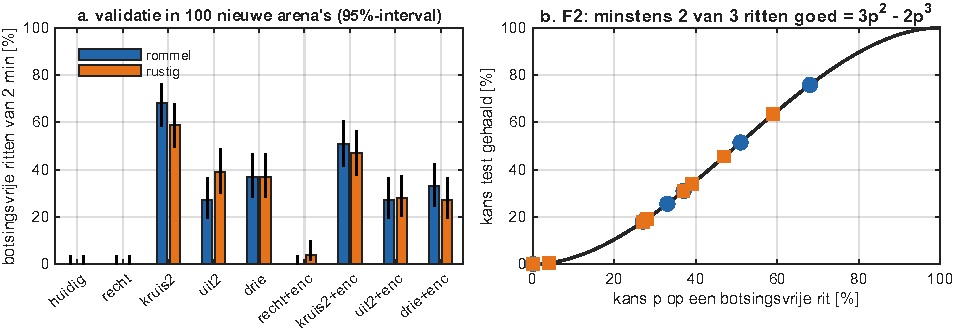
\includegraphics[width=\textwidth]{obst_resultaat.pdf}
\caption{(a) Botsingsvrije ritten per opstelling in nieuwe arena's. (b) Van kans per rit naar kans dat de
F2-test slaagt.}
\label{fig:obstres}
\end{figure}

\begin{figure}[H]
\centering
\begin{minipage}[t]{0.47\textwidth}\centering
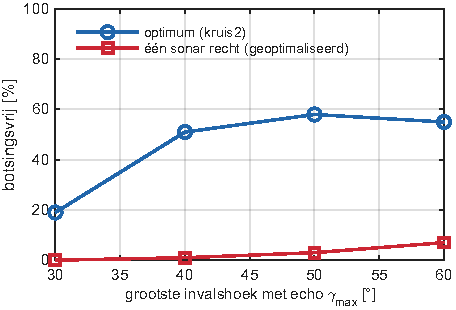
\includegraphics[width=\textwidth]{obst_gamma.pdf}
\caption{De uitkomst hangt sterk af van $\gamma_{\max}$: van \ObstGamDertig~\% bij 30° tot
\ObstGamZestig~\% bij 60° voor het optimum.}
\label{fig:gamma}
\end{minipage}\hfill
\begin{minipage}[t]{0.50\textwidth}\centering
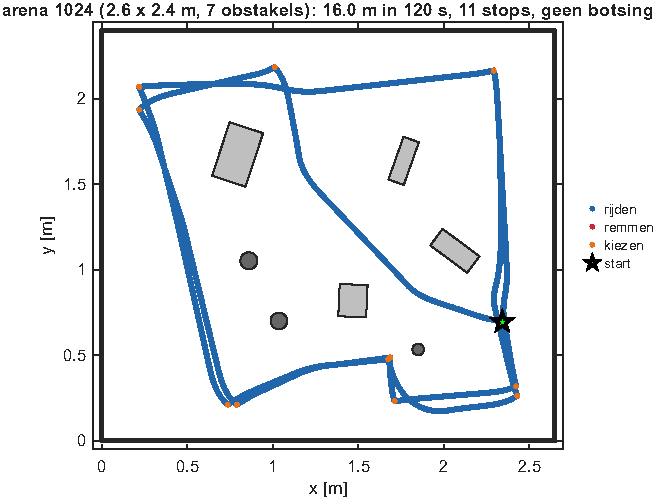
\includegraphics[width=\textwidth]{obst_rit.pdf}
\caption{Een rit van het optimum; kleur = toestand.}
\label{fig:rit}
\end{minipage}
\end{figure}

% =====================================================================
\section{Wat dit betekent voor het ontwerp}
\begin{enumerate}[leftmargin=6mm]
\item \textbf{Lijnsensor}: vier kopjes op een steek van \LijnBestSteek~mm, \LijnBestL~mm voor de
  aandrijfas; alles tussen 45 en 80~mm en een steek van 8 tot 15~mm is vrijwel even goed. De losse
  kopjes van een 4-kanaals tracker kun je vrij plaatsen. Wordt de tape 10~mm, zet de steek dan op
  $w/1{,}5 \approx 7$~mm.
\item \textbf{Lijnregelaar}: dit is waar de winst zit. PD met gefilterde D-term op 200~Hz, instellingen
  hierboven; begin op de echte auto met deze waarden en stel alleen $K_p$ en $v_{\max}$ bij. Wie
  voorzichtig wil beginnen: de analytische $K^* = 2v/L^2$ geeft de kleinste afwijking (12~mm), maar is
  anderhalf keer zo traag.
\item \textbf{Sonar}: gebruik beide bestelde HC-SR04's voor F2, gekruist: de linker kijkt
  \ObstAlfaKruisLo--\ObstAlfaKruisHi° naar rechts en omgekeerd (de simulatie koos \ObstBestAlfa°).
  Laat ze om de beurt vuren.
\item \textbf{Motoren}: kalibreer een trimfactor per motor (F2.1 vraagt $\le$\,\ObstDeltaMax~\%
  verschil). Encoders gaven in deze simulatie geen aantoonbare winst voor F2 (tabel~\ref{tab:obst}),
  maar maken draaien over een vaste hoek wel nauwkeurig.
\item \textbf{Remmen}: kortsluitrem (IN1 = IN2 met EN hoog), nooit uitrollen.
\item \textbf{3D-model}: maak de overhang achter de as korter of de achterkant rond (zwaaistraal).
\end{enumerate}

\section{Wat eerst gemeten moet worden}
Een simulatie is zo goed als de getallen die erin gaan (Mouret \& Chatzilygeroudis 2017). De getallen
met [AANN] in \texttt{qdat\_parameters.m} zijn schattingen; de eerste vier zijn het belangrijkst:
\begin{enumerate}[leftmargin=6mm]
\item $\gamma_{\max}$: zet de auto op 30~cm voor de muur en een kist, draai hem in stappen van 5° en noteer
  tot welke hoek de HC-SR04 nog een echo geeft. Dit getal bepaalt de uitkomst van F2 het meest
  (figuur~\ref{fig:gamma}).
\item Dode zone en $v_0$: laat de PWM langzaam oplopen tot de wielen draaien; meet de snelheid bij
  PWM 255 over 2~m.
\item $\tau_m$ en remweg: film een noodstop vanaf 0,3~m/s naast een meetlat; vergelijk met
  \eqref{eq:rem}.
\item Lichtvlek $\sigma$: schuif een sensorkopje dwars over de tape en log de analoge waarde; pas
  \eqref{eq:dekking} erop.
\end{enumerate}
Het eigenlijke resultaat van dit onderzoek is dan het verschil tussen simulatie en werkelijkheid in
meetbare eenheden: rijd hetzelfde parcours met dezelfde instellingen en vergelijk rondetijd en
$e_{\max}$ met tabel~\ref{tab:val}.

\section{Bestanden}
\begin{center}\footnotesize
\begin{tabular}{@{}ll@{}}
\toprule
bestand & functie \\
\midrule
\texttt{qdat\_parameters.m} & alle maten en aannames, met bron \\
\texttt{onderzoek\_lijnvolgen.m} & simulatie 1: kaart, varianten, validatie, figuren (\LijnDuur~min) \\
\texttt{onderzoek\_obstakels.m} & simulatie 2: analyse, optimalisatie, validatie, figuren (\ObstDuur~min) \\
\texttt{demo\_lijnvolgen.m}, \texttt{demo\_obstakels.m} & 3D-weergave van een rit, optioneel als MP4 \\
\texttt{model/} & rekenkern: voertuig, sensoren, banen, arena's, beide simulaties, 3D-model \\
\texttt{optimalisatie/} & kostfuncties, random search, validatie \\
\texttt{resultaten/} & figuren en \texttt{.tex}-bestanden met de getallen voor dit document \\
\bottomrule
\end{tabular}
\end{center}

\begin{thebibliography}{9}\footnotesize
\setlength{\itemsep}{0pt}
\bibitem{bra} V.~Braitenberg, \emph{Vehicles: Experiments in Synthetic Psychology}. MIT Press, 1984.
\bibitem{han} N.~Hansen, ``The CMA Evolution Strategy: A Tutorial'', arXiv:1604.00772, 2016.
\bibitem{jak} N.~Jakobi, P.~Husbands, I.~Harvey, ``Noise and the Reality Gap'', ECAL 1995, LNCS 929, pp.~704--720.
\bibitem{leo} J.\,J.~Leonard, H.\,F.~Durrant-Whyte, \emph{Directed Sonar Sensing for Mobile Robot Navigation}. Kluwer, 1992.
\bibitem{mou} J.-B.~Mouret, K.~Chatzilygeroudis, ``20 Years of Reality Gap'', GECCO '17 Companion, pp.~1121--1124.
\bibitem{sie} R.~Siegwart, I.\,R.~Nourbakhsh, D.~Scaramuzza, \emph{Introduction to Autonomous Mobile Robots}, 2e dr. MIT Press, 2011.
\bibitem{tob} J.~Tobin e.a., ``Domain Randomization for Transferring Deep Neural Networks from Simulation to the Real World'', IROS 2017, pp.~23--30.
\bibitem{wes} T.~Wescott, ``PID Without a PhD'', \emph{Embedded Systems Programming}, okt.~2000.
\end{thebibliography}

\end{document}
